\documentclass[fleqn,10pt]{wlscirep}
\usepackage[utf8]{inputenc}
\usepackage[T1]{fontenc}
\usepackage{gensymb}

\title{Drought variability structures social interaction in the prehistoric American Southwest}

\author[1,*]{Nicolas Gauthier}

\affil[1]{School of Human Evolution and Social Change, 900 S Caddy Mall, Tempe, USA}

\affil[*]{Nicolas.Gauthier@asu.edu}

\keywords{Archaeological Networks, Spatial interaction model, Drought}

\begin{abstract}
  In agrarian societies, social networks help absorb weather-related shocks by facilitating resource flows to afflicted settlements and population flows away from them. This property of social networks depends on the degree to which the network can connect populations in topographically accessible locations that tend to experience different weather patterns. We thus expect rainfall covariance in space and time to interact with patterns of landscape connectivity to structure prehistoric social networks. Here we analyze 7.5 million archaeological artifacts recovered from 500 sites in the precontact American Southwest, and estimate how the intensity of social interaction varies as a function of distance and growing-season aridity. We find that the intensity of social interaction in the past is highly distance dependent. We also find that social interaction between regions experiencing different domains of externally-forced drought variability (e.g. Pacific vs Atlantic dominated) is higher than would be expected by distance alone, while that drought patterns arising from internal variability do not impact network formation. Our findings are add empirical detail to ideas long theorized in anthropology, while emphasizing the need for more precise definitions of ``climate'' in studies of human-environment interaction in the past. and will be useful for projecting potential social responses to drought events in the past and present.
  \end{abstract}

\begin{document}

\flushbottom
\maketitle


\thispagestyle{empty}


\section*{Introduction}

1. why this study is needed (preview background)
In times of drought and famine, farmers in dryland environments turn to their social networks to avoid starvation.

%Food transfers among farmers link the food supplies of distant settlements. Similarly, atmospheric transport of moisture via local evapotranspiration and re-precipitation can sync crop yields across distant agroecosystems. 

%Tracing the flows of food, water, and energy within these complex social-ecological systems is essential for understanding their long-term behavior, and leveraging our archaeological understanding of why societies succeed or fail will be critical to anticipating the impact of impending climate changes on farming communities in the developing world.

--given a known pattern of environmental variability, how can we anticipate specific cultural responses?

Archaeology -- because of its focus on the material correlates of human behavior over long time spans -- is uniquely suited to address how social and physical infrastructure modulates human interactions with the environment. Not only do archaeologists catalogue the remains of field systems, road networks, canals, and other components of hard infrastructure directly, but also the ceramics, raw materials, and luxury goods that are the material correlates of networks of exchange and interaction.
A central principle in archaeology is that we can use the spatial and temporal patterns of environmental variability to predict ideal cultural responses, and then compare those expected patterns to observed ones to test the importance of that particular pattern of environmental variability. \cite{halstead1989}. This process gives archaeologically testable empirical implications -- that people will interact with people who have a different risk profile. The physical environment defines the costs and benefits of social interaction, and provides the structuring context in which human decision making occurs.

2. what this study does/finds (preview methods/findings)
Rates of site preservation and recovery are exceptionally high in this region. Nearly two centuries of survey and excavation have yielded extensive, high quality settlement pattern data.
Late pre-Hispanic US Southwest -- Detailed inventories of material culture at more than 500 archaeological sites provide an unparalleled view of the structure and dynamics of past social networks, and the climate of this period has been intensively studied by paleoclimatologists and climate modelers. Here, I will use statistical models to isolate robust social and environmental *patterns* at the macro-scale.

The goal here is to extract ROBUST patterns of climate variability, moving beyond the small-scale point based year to year correlations. The latter can easily be dominated by noise or other issues with sampling variability. The method we use here yields similar results in appearance, but in a more objective fashion designed specifically to skillfully extract signal from noise.

spei is independent of local climatology. Alternatively, we can think of patterns of interannual variability. After holding mean climate constant, we look at the pattern of excursions from that mean value for each region. So it doesn't matter if you are comparing a wet and dry location, what's important is whether each location is wetter or dryer *than average for that location* at similar times.

Note that we refer to the full range of moisture/ aridity variability here as drought for concreteness and simplicity.The central idea here is that drought and pluvials. For simplicity we refer to these as modes of ``drought'' variability, but note that the SPEI measure captures the full spectrum of hydroclimate variability, from extreme drought and pluvial events to finer variability in moisture and aridity. The key point is that all this variability maps onto similar spatial modes, due to their reliance on the same underlying atmospheric dynamics.

To our knowledge this study is the first of its kind to apply gravity models in their statistical incarnation to archaeological data. This complements ongoing work in the simulation of gravity style spatial interaction models  in archaeology (cite wilson, bevan et al), and opens the door for a more rigorous evaluation of dynamical theories against the empirical archaeological record.
Although gravity modeling was for a time populat in archaeology and anthropology (johnson, hodder, tobler) it has less use in recent years. But now we have large regional databases which much better chronological control.

3. what this study contributes (preview discussion)
By combining first-principles modeling with extensive empirical datasets, the proposed research is of a kind sorely needed in the ongoing study of sustainability in social-ecological systems. This interdisciplinary modeling framework, and the insights generated with it, will be of use not only to archaeologists, but also to anthropologists, development economists, and the broader climate-change impact-assessment community by making tractable problems with hidden, non-trivial human-environmental linkages.

We explore the dynamics of social networks as social infrastructure, a set social relationships for redistributing food, people, and information that increases the robustness of human populations to environmental variability.

\section*{Background}
Recent theoretical and empirical work has begun to address how spatial, social, and environmental factors structure exchange networks \cite{Nolin2010Food-SharingIndonesia,Koster2014,Hao2015,Schnegg2015}. Exchange systems are not independent of the environment, and the biophysical context of exchange is an important component often ignored in the anthropological literature. A more general approach to these systems views them as a form of social infrastructure, channeling the flow of energy between spatially structured populations in much the same way as food webs channel energy in ecosystems \cite{Crabtree2015,Crabtree2017ReconstructingStates}.

Infrastructure is the filter through which humans interact with their environment \cite{Anderies2015}. A farmer, for example, does not interact with rainwater directly but instead uses systems of canals and fields in coordination with a network of other farmers to manage flows of water in space and time \cite{Yu2015}. Canals, roads, and other forms of physical infrastructure enable physical flows like water and people. Social infrastructure channels information, and provides affordances for additional mass and energy flows \cite{Anderies2015}. At their core, exchange networks are clusters of social relationships that redistribute food, people, and information among a structured population of agents. These relationships are a form of public, social infrastructure because they enable the transfer of matter, energy, and information between populations of potentially distant resource systems. Social networks are both intangible and irregularly mobilized, requiring significant investment to maintain and monitor. As is the case with physical infrastructure, social networks will degrade over time if not actively maintained.

Social infrastructure interacts directly with physical infrastructure because social networks often must map onto spatial networks. Metabolic costs, such as the energy expended producing and transporting food over space, provide constraints on energy flows in exchange systems \cite{Drennan1984}. In any particular case, the balance between these costs and the metabolic benefits of social interaction influences whether resources are moved in bulk to populations in need, or whether those populations move themselves to the available resources. The topology of spatial networks also constrains who can interact with whom, introducing bottlenecks and other structural flow constraints \cite{Barthelemy2011SpatialNetworks}. Improvements to transportation infrastructure, such as roads and trails, decrease the effective distance between different settlements; failure to maintain these transportation networks increases the effective distance \cite{McCall1985TheAfrica}.

A canal system cannot be understood in isolation from local weather and topography, and neither can an exchange system. An idealized food-transfer network (i.e., lacking physical or social constraints) acts as a spatiotemporal **low-pass filter** on environmental noise, meaning that farmers in the network receive the space-time average crop yields given variable rainfall \cite{Harpending1977}. An understanding of the patterns of variability in rainfall, in particular how rainfall covaries across different nodes in the network, will thus provide a insight into the kinds of environmental pressures that drive food-transfer systems. The **social-ecological network** concept is useful tool for understanding how social networks fit into a such a broader ecological system.

%  The benefits of interacting with populations experiencing predictably distinct drought patterns are obvious. Social networks allow for the flow of information between spatially distinct populations, allowing agents to monitor conditions in other places, allowing them to target locations for trade or migration.

% The benefits of social interaction in this context include information, resources and trade, food exchange, migration, marriage. Costs include metabolic costs, social costs of moving through unfriendly territory, water, time and related opportunity costs, difficulty of monitoring cooperation and sanctioning free riders, and imperfect information about where best to go. cite rautmann for idea that actual volume of food is less important that information.

% benefits of maintaining social relationships




\section*{Case Study}

Here, I use an empirical archaeological case study to explore interactions between food exchange and ecohydrology: the late pre-Hispanic American Southwest. These regions both span areas of about 460,000 square kilometers centered on latitude 35\degree N, the rough limit of the subtropical ridge that determines the northern extent of the world's hot deserts. Winter rainfall is delivered by large-scale precipitation and mesoscale storms brought by westerly winds, and summer precipitation falls from convective storms associated with southerly Monsoonal winds. Rainfall in both seasons varies markedly year-to-year and, because the majority of annual precipitation can fall in only a handful of storms, it is highly unpredictable in space. Multidecadal drought conditions are common in these regions. Global atmospheric teleconnections often initiate drought conditions -- unusually cool Pacific sea surface temperatures (La Ni\~{n}a phase of the El Ni\~{n}o-Southern Oscillation) in the American Southwest. Interactions between the land and atmosphere are also strong \cite{Koster2004RegionsPrecipitation}, so the length of these dry spells often reflects more localized positive feedbacks between vegetation and soil moisture \cite{Ault2014AssessingData}. Vegetation growth in semiarid environments is water limited, but vegetation itself is often a major source of this  water because of terrestrial moisture recycling. Humans in these regions not only depend on these feedback loops -- soil moisture constrains cereal agriculture as much as natural vegetation -- but also play an active role in them through deforestation and irrigation.

Human populations in these environments have developed similar suites of social and physical infrastructure to manage environmental risk. Food storage is one effective strategy for preserving bulk grains in dry environments, and storage features are a common archaeological find \cite{Spielmann2011SustainableEnvironments}. Irrigation, in particular via runoff harvesting infrastructure near seasonally flooded streams (**wadis**/**arroyos**), redistributes soil moisture in space and time to create microenvironments for agriculture. But these systems are vulnerable to flooding and would have demanded significant labor investments to monitor and maintain \cite{Shaw1982, Dominguez2005,Beckers2013AncientAsia}. Such strategies would have been effective for managing small-scale variability (year-to-year and field-to-field), but would have been vulnerable to a long-lasting, spatially extensive droughts and pluvials \cite{Halstead1989}. During such extreme weather events, inhabitants of these regions must mobilize social networks to -- depending on the scale and severity of the event -- move food to afflicted settlements or move people away from them. The precise nature of these social networks, and the means by which this social infrastructure was provisioned, varies substantially between cultures and time periods. But the costs and benefits that go into individual decision making are more static.

The populations of the late pre-Hispanic period in the American Southwest subsisted mainly on maize production, supplemented by a mix of beans and wild proteins. Food transfers are thought to have occurred primarily in the context of informal sharing within kin groups, reciprocal exchange at ritual ceremonies and festivals, and residential mobility on the scale of one to three generations \cite{Hegmon1991,Hegmon1996,Kohler1996TheAnasazi,Varien1999SedentismBeyond,Cordell2007MesaMigration}. The archaeological record attests to extensive exchange networks of durable goods such as ceramics and obsidian \cite{Mills2013a}, and there is direct (if limited) evidence for the long-distance transport of maize \cite{Benson2009PossibleMexico,Benson2010WhoDrought}. There is also evidence for long distance migratino (TODO cite mills again?)

\begin{figure}[ht]
\centering
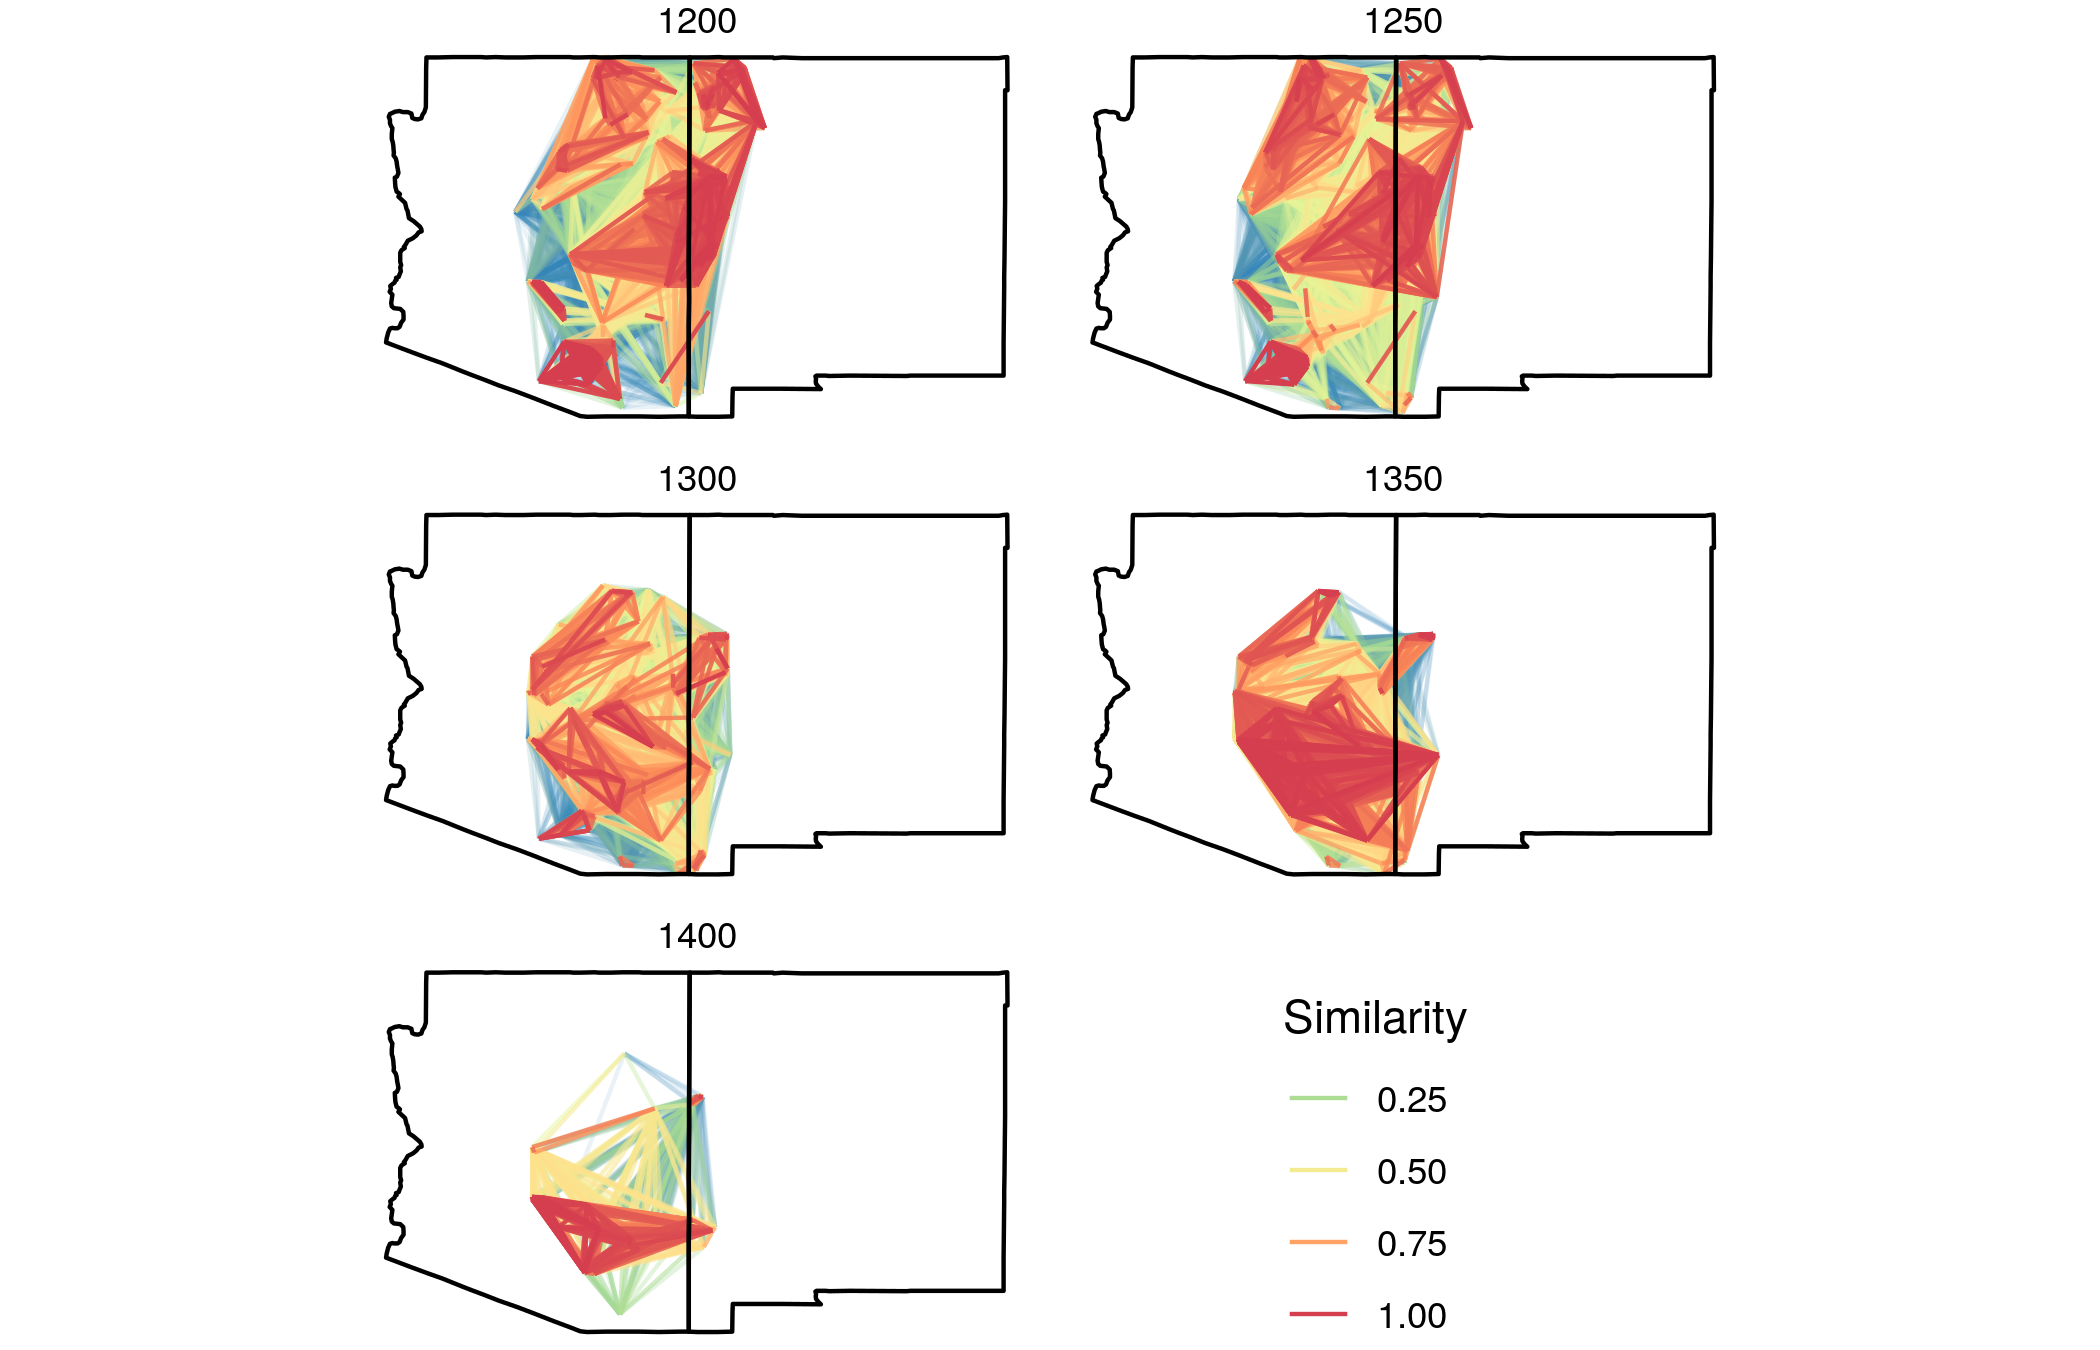
\includegraphics[width=\linewidth]{figures/similarity_network.png}
\caption{The \emph{Southwest Social Networks} dataset, version 1. Each line connects two archaeological sites. The color of the line represents the similarity of artifacts recovered from the pair. A BR coefficient of 1 means the sites share the exact same decorated ceramic wares in the exact same proportions, and a coefficient of 0 means there is no overlap in the ceramic assemblages. This similarity network can be interpreted as the degree of social interaction and cultural transmission between sites, whether via migration, trade, or copying. Networks are shown over successive 50 year time spans, starting at 1200 CE. A relatively stable network configuration starting at 1200 CE is interrupted by climatically-forced migrations near the end of the 1250 time step.}
\label{fig:network-plot}
\end{figure}



This is a common qualitative observation in many anthropological and archaeological studies of traditional societies (scudder1962, cashdan 2001, waddel 1975, colson 1979, speilmann 1982, 1986, cashdan 1985, wiessner 1982, werner 1983, yengoyan 1972, duff 1998, 2002, cameron 1995, jaskoff and adams 1977, crumly 1979).



Cordell et all investigated theimpact of preciptaion variability on ceramic exchange in tenth-thirteenth century mesa verde. They highlight a bimodal precipitation regime, extracted from a PC analysis of 28 tree ring cronologies form 689-1988. They suggest that broad ceramic regions examined by archaelogists reflect "maximal risk sharing networks."
--how's what im doing different -- braoder climatedata, much more robust spatial sampling, much more extensive quantitative

Rautmann focused on central new mexico, 900 - 1259. Using BR similarity coefficient and local weather station precipitation data, she found networks up to 50km away. This is consistent with greater ineraction within 80km due to spacing required to maintain viable breeding population she says. She highlights differential ``investment of social energy in the maintenance of social ties between the two areas''

Strawhacker et al looked at risk landscapes in the mimbres region. The used tree-ring based reconstructions of interannual precipitation variability, and sought to determine the extent to which sites interacted with those that experience negatively correlated rainfall patterns.
year to year correlations can contain considerable noise that might mask real time-invariant patterns of interannual variability. Plus using linear correlation coefficient's on rainfall data, as deviations from normality in the tails of the distribution can potentially bias estimates of extreme events. Furthermore, water availability for food production is not merely determined by rainfall, but by the relative rate of precipitation to evaporation, which is itself partially determined by factors such as temperature, wind speed, and humidity.

Social networks are survival networks uses the same dataset here, but different because ....
They note that both Zuni and Hopi survive drought

There have been fewer qualitative tests of these patterns in anthropology (with some notable exceptions (Strawhacker, cordell, rautman, johnson)). This study seeks to extend the findings from these specific works to the greater Southwest region, using a much richer collection of social and environmental data and theory informed by complex systems.


--TODO do i need to discuss past least cost path papers in the southwest? probably.

% Spatial interaction models and social gravity
chester king, 1976, 289-290 is source of idea that "the greater the difference between thet wo resource areas, the greater the intensity of economic interaction and the greater the number of social bonds, including marriages"

Johnson actually fits a gravity model to chumash marriage data
The use or gravity style statistical models is uncommon in archaeology, with exceptions (johsnon, others he cites). The method is becoming popular in archaeology from a dynamical perspective, but not yet from a statistical perspective.
He finds some evidence for increased marriages between different average climate zones (coastal and inland) but the effect is weak compared to distance and  size

Tobler cappadocian speculation uses it too

To our knowledge this study is the first of its kind to use social gravity models on archy data from statistical perspective




Shared
"regional styles of elaborate ceramic tableware suggest a major role for commensality in cultivating relationships of solidarity, bothwithin and between settlements (e.g., Tomkins, 2007; Urem-Kotsou
and Kotsakis, 2007)." -- talk about this in the context of ceramic similarity -- tablewares important because they speak to ocmmensalism and feasting

\section*{Results}

\subsection*{Distance Decay of Social Interaction}
Our null hypothesis, that distance alone is sufficient to explain the observed divergences between archaeological assemblages, was sufficient to explain nearly 50\% of the variability in our dataset. 

The functional form of this distance decay closely resembles the taylor function, a combination of the traditionally used exponential and power distance deterrence functions. This represents that multiple transmission processes, with different relationships to distance, are acting together to generate the variation we see in the archaeological record.

The two main inflection points in the decay curve are both consistent with previous work in the ecology of human movement. The threshold of 1 hour, below which distance has no effect on social interaction, is consistent with Marchetti's constant, which states that the average journey to work time is ~30 minutes cross culturally. This reflects that distance is much less of a factor between settlements within a day's walk round trip of one another, suggesting that the distance deterrence only becomes a factor dealing with purposeful multiday trips. 

The second inflection point, at roughly 5 hours or 80 km, is consistent with estimates of area needed to sustain the minimum viable breeding population for human groups

\begin{figure}[ht]
\centering
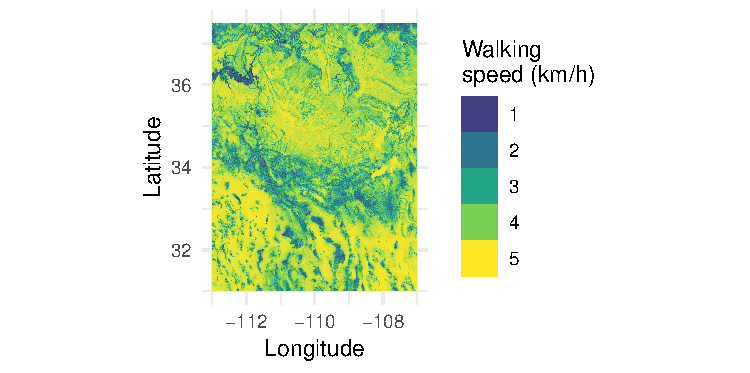
\includegraphics[width=.8\linewidth]{figures/walking_speed.pdf}
\caption{Estimated terrain-mediated walking speeds in the US Southwest study area. Speeds calculated from terrain slope (percent) using a modified version of Tobler's hiking function that decreases the perceived speed of traveling across very steep slopes.}
\label{fig:walking-speed}
\end{figure}

Look at distance cutoffs, are they consistent with the figures of 50km-80km from rautman and drennen and others? johnson finds no marriages past 60km, maize to chaco papers also have distance figure of 80km

"plateu effect" or distance within which distance doesn't matter, from johnson but cites olsson 1965 and crumley 1979. also cite ariadne distance deterrence function for similar idea
~5km should be the ticket if marchetti's constant holds

We see in figure \ref{fig:walking-speed} that the mountainous terrain adds considerable spatial variation to potential walking speeds. When this topography is translated to paths, we see how the Mogollon Rim acts as a severe bottleneck for spatial flows, with paths generally constrained to one of the three river systems, the Verde, Salt, and Gila, act to channel flow across this boundary.  

\subsection*{Spatial Modes of Drought Variability}

The rotated PCA analysis reveals four leading modes of variability, which collectively explain 77\% of the variability in the 106 year observational record. represent the influence of Pacific sea surface temperatures, and associated anomalies such as El Ni\~no Southern Oscillation and the Pacific Decadal Oscillation. The fourth and fifth empirical orthogonal functions represent internal atmospheric variability, associated with regional circulation patterns not influenced by the pacific.

These spatial and temporal drought patterns, and their hypothesized forcings from the global climate system, are largely consistent with those from other studies using varied observational data and time windows (cook meko et al 1999 j climate, mccabe et al 2004, mccabe and dettinger 1999, dean et al,)

leading reof looks like el nino, resembles southern oscillation pattern (antiphase) from mccabe and dettinger 1999

distinguish between forced spatial patterns from ssts and those that are spatilly coherent internal variability, "noise" in some sense, but distinct from the spatially incoherent variability (TODO cite ault? pc paper)


resembles varimax rotate pcs from cook meko et al 1999 j climate -- summer pdsi variability

\begin{figure}[ht]
\centering
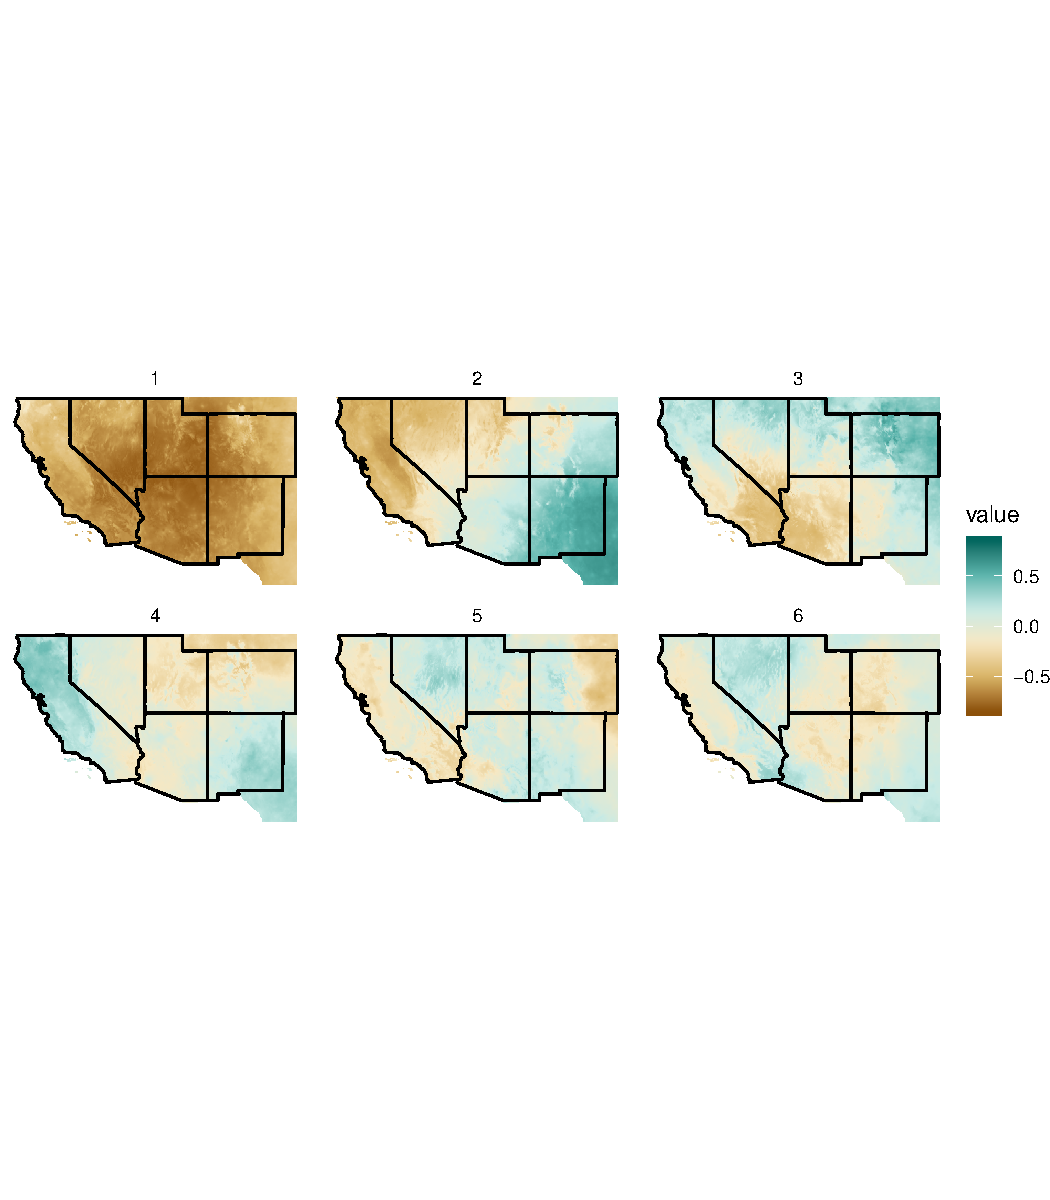
\includegraphics[width=.8\linewidth]{figures/eof_observed.pdf}
\caption{Leading 4 rotated empirical orthogonal functions. The empirical orthogonal functions are the spatial patterns associated with their respective principal component time series. The EOFs are the eigenvectors of the space-time covariance matrix, and the PCs are the eigenvalues. The leading four EOFs, which together explain 77\% of interannual drought variability in the observational record, were then subjected to varimax rotation, to make the spatial patterns more physically meaningful by relaxing the spatial orthogonality constraint.}
\label{fig:reofs}
\end{figure}

REOF1 represents a center of action in the desert Southwest portions of California and Arizona, extending up to the northeast. It represents the influence of tropical Pacific sea surface temperatures, such as the North American Monsoon, late-summer tropical storms, and more broadly ENSO variability. This pattern is produced by southwesterly flow from the tropical pacific, bringing moisture up across the low desert zones. The pattern attenuates with gains in elevation, as distance from the ocean increases. 

REOF2 similarly represents southeasterly flow from the Gulf of Mexico, with a center of action in eastern New Mexico. As with REOF1, the pattern attenuates with increasing elevation and distance from the ocean, due to orographic and continentality effects, respectively. It represents cyclonic storms coming from the Gulf of Mexico, in turn influenced by variability in Atlantic sea surface temperatures. 

The pair of Pacific and Atlantic SST dominated drought patterns in the Southwest has been previously hypothesized before in the context of archaeological change (dean and van west), but the level of spatial detail here far surpasses previous studies. There in the context of a ``bi-modal precipitation distribution'', meaning the distinguishing between regions with both summer and winter dominate precipitation (REOF1) and those with just summer dominate precipitation (REOF2). Although specifically growing season (summer) variability is measured here, the pattern is also consistent with winter moisture variability, as the 12month SPEI index integrates the long lag effects of winter moisture, and the summer and winter patterns are governed by similar atmospheric teleconnections to Pacific SST variability.

the leading 2 specifically show up  in cook and meko
Gulf of Mexico, and by extension Atlantic ssts and whatnot

REOF3
Colorado plateau

REOF4 clearly represents the influence of westerly flow off the Pacific Ocean, and the orographic effect of the Sierra Nevada mountains intercepting this flow.

These leading modes represent spatially coherent variability. The trailing modes which were not retained for rotation represent spatially incoherent (i.e. random) variability. We can further decompose the spatially coherent modes into those that are externally forced, due to variability in Pacific SSTs, for example) and those that represent variability internal to the Western US climate system.

These same patterns from the observational period also show up using the reconstruction, pulling in data from 1100 CE to present. This underlies the fact that these are robust, time invariant spatial modes. The correlation between the amplitude time series for matching spatial patterns was XXX

% temporal reconstruction

\subsection*{Spatial Interaction Modeling}

here talk about best fitting models and whatnot.




\subsubsection*{Drought Variability and Social Interaction}

\begin{figure}[ht]
\centering
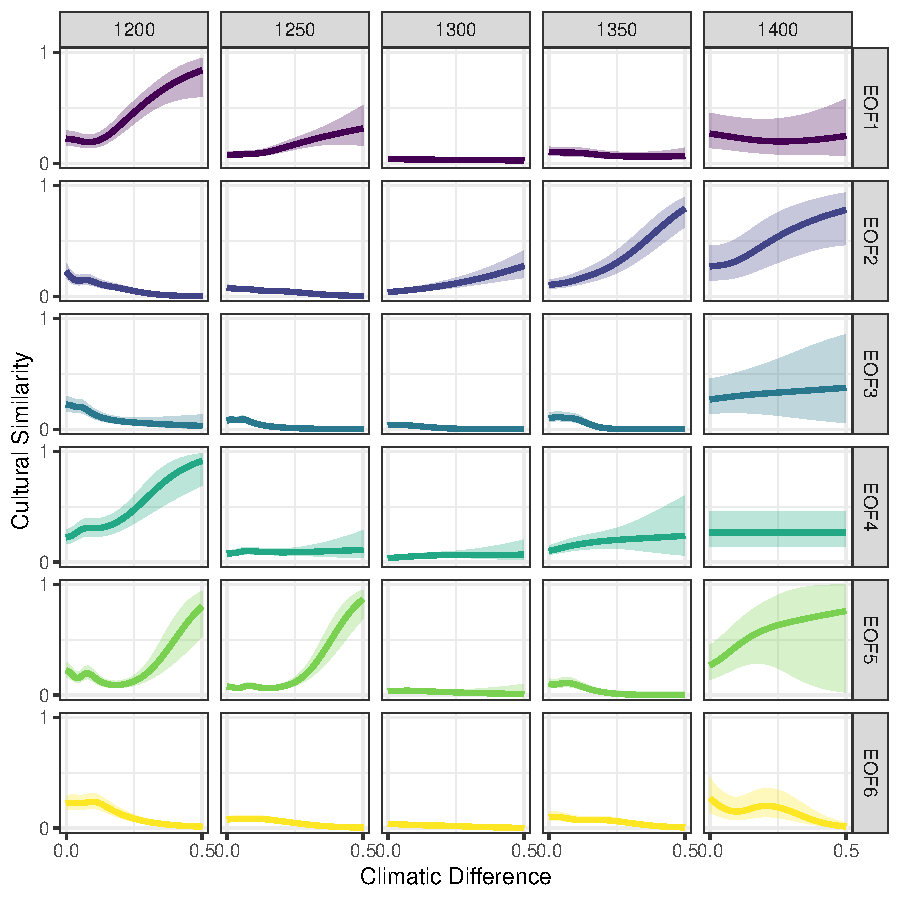
\includegraphics[width=.8\linewidth]{figures/smooths.pdf}
\caption{Estimated smooth functionals.}
\label{fig:smooths}
\end{figure}

interpret relative r2 -- in johnsons chumash paper r2 was .43 for distance and size, and adding dummy variable for same or different enviroment only increases model to .44

do negative interactions (ie low) point to raiding and conflict?

zuni and hopi

changes in rho value over time -- pointst tomore idiosyncratic interaction

Up to three levels of \textbf{subheading} are permitted. Subheadings should not be numbered.

\section*{Discussion}


points to disucss:
1. Why doesn't size matter?
2. Why do things change over time?
3. What does ceramic assemblage similarity even mean?
3b. fully connected widhgted network, but what if pruned?
  we argue here our approach here is appropriate because we are aggregating many, sparse social networks of individuals together at the population scale. that is we look at macroscale flow patterns given microscale social networks, maxent approach means we make the fest possible assumptions about the configuration of the microscale social networks
5. Importance of asymmetry. citing crabtree talk about asymmetric debts. also talk about differences in population size and gravity model. what do we miss out on when use symmetric data?
4. zuni and hopi? seemingly different because different external vs internal tie patterns, but actually they both cross climate zones
6. we just looked at summer growing season, but what about winter (where bimodal)? Site coates et al 2015 for variability in the seasonal phasing of rainfall
7. We don't look at the role of drought in producing similarity, such as a drought leading to many migrants, but rather look at long term patterns in the differences. This is because we integrate out the mean of each site to get attractiveness, effectively integrating out utility measures (bavaud 2002, 2008). So we are specifically looking at the "deterrence" effect of claimate distances, that is the costs and beneftis of interaction.

cordell et al he argue that this pattern breaks doesn ca 1239-1488, and explain it as the source of disruption in this period as the social networks that developed to cross it over the centuries were not able to adapt in time to the temproariliy distinct precipitaiton regime. -- this is an important point, and why networks aren't always just optimally minimizing correlation, they take time to build and effort to maintain, especiailly on the time scales greater than a singel generation. so they are specifically forming in response to robust patterns of variability. In the future it will be important to model the evolution of paths separately, a la bevan and wilson, in order to capture this time lag effect.

This study sought specifically to investigate the impact of effective distance and drought variability using statistical models, specifically focused on the functional forms of these relationships. Future study will leverage these findings to construct dynamic simulation models. This will allow us to capture year-to-year variability, as well as the time averaging and bias introduced by archaeological investigation.

%Qualifications, Caveats, and Future Work
jensen inequality, E(logit(y)) >=logit(E(y)). this means we should interpret specific predictions and confidence intervals from this model with caution, and instead only focus on interpretaiton of the brod functional forms. Its a necessary evil here, becuase we do not yet have the computational abiliy to fit the corMLPE correlation structure and a beta family. Preliminary tests with the data suggested that the pairwise correlation structure was a much alrger source of bias then transforming the response variabble,so that's the tradeoffwe went with. The bias from transforming the respone leads to bias in the estimates of variance

the eof patterns are in part scale dependent. Thihs iss isnt necesarily a problem, its a necessity that the answer to the question what kind of variability matters is inherently tied to the scale at which on asks the question, there are no right or wrong answers. Although the particular choices of variables, resolution, domain size, truncation level, were informed here by theory and tested to as to minimze sensitivity to paritcular choices made by the authors, different researchers could still generate equally resonable results given  different input parameters.  This is simply to state that the drought patterns highlighted here, while we are confident they are not statistical artifacts, should be used with caution in contexts outside of the specific context here.

Simulation type models address these questions, summarize results and say what this adds to them, and more broadly why empirical investigations such as this complement them.
This problem has been the focus of many computaitonal simulations. risk sharing works in pooling network for need based transfers(hao et al 2015) but a key factor was how well eveyrone knoew everyonelses wealth. this is acost od distance, further away you are the les you can monitor others for free riding
janssen pop aggregation shoes climate variaiblity impacts short term aggregation, resource dynamics long term population levels, exchange cricial for maintianin populatiopn levels, sharing leads to short term stability but long term degredation

hegmon - resricted sharing?

crabtree -- importance of asymmetry of debt and obligations -- from this perspective eof's are optimal because you are most guaranteed to minimize the asymmetry of your dbts

anderies and hegmon -- information contstaints important for migration, need to know that your potential migration destination is actually a good place to go, because if you go and you were wrong (its jsut as bad) then thats a big costs. errors in information, such as over distance, make people more likely to move when its actually a bad aidea and fwer to move when its a really good idea

anderies nelseon and freeman - exchange resources with different risk profiles -- even in wet environments, and increase in interannual variability will decrease the robustness specialist food supply in variation to rainfall -- so ag economy based on specialization is more limited by interannual deviations than mean amount

\section*{Methods}


\subsection*{Spatial interaction model}

We start with a symmetric similarity matrix $\mathbf{T}$ with elements $T_{ij} = T_{ji} = BR_{ij}$ with $BR$ defined as the scaled Brainerd-Robinson coefficient of similarity between the proportions of decorated ceramic ware types.

$$BR = 1 - \sum_{k=1}^{p} \lvert P_{ik} - P_{jk} \rvert$$

where $P_{ik}$ is the proportion of ceramics of type $k$ at site $i$.

This metric estimates the similarity in the ceramic discard assemplages between pairs of sites, which in turn is a proxy for cultural preferences, food consumption differences, access to raw materials, and access to trade networks. The index can be loosely interpreted as a probability of interaction between two sites, with identical patterns of ceramic discard indicating a high likelihood of interaction via either direct migration or trade or indirect cultural diffusion.

This is a standard metric in archaeology (cowgill 1990, golitko et al 2009, hart engelbrecht 2012), similar to the xy distances used in other fields, and is used to .

We fit models of the form

$$T_{ij} = k v_i^\mu w_j^\alpha \exp(\beta c_{ij})$$

where $c_{ij}$ is some notion of the generalized cost of moving from $i$ to $j$ and is symmetric, meaning $c_{ij} = c_{ji}$.

Gravity models of this form are quasisymmetric, and can be decomposed into symmetric and asymmetric components


Which states that the flow of people, goods, or information from site $i$ to site $j$ is a function of some property $v$ of site $i$, property $w$ of site $j$, and the distance between them $c_{ij}$ with $c_{ij} = c_{ji}$

A key question is how to relate directed, asymmetric flows in $T_{ij}$ to the undirected, symmetric similarities in $BR$, that is what is $BR = f(T_{ij},T_{ji})$, which is to say how does ceramic assemblage similarity reflect the underlying flow of people, goods, and information?


Question: Do regional interaction networks self-organize with respect to patterns of climate variability, and if so at what spatial scales does this organization occur?

Social networks help absorb weather-related shocks by facilitating resource flows to afflicted settlements and population flows away from them. This property of social networks depends on the degree to which those networks can connect topographically accessible locations that tend to experience different weather patterns. I thus expect patterns of rainfall covariance in space and time to interact with patterns of landscape connectivity to structure prehistoric social networks.

This relationship has been documented in the US Southwest on smaller spatial scales, using definitions of ``climate variability'' limited by the environmental data available in each case \cite{Rautman1993a,Cordell2007MesaMigration,Strawhacker2017RiskProvince}. The proposed work expands on these efforts to analyze the entire regional system, using two types of climate variability derived from a paleoclimate model-data fusion technique.

\subsection*{Archaeological Social Network Proxies}

I draw on an extensive archaeological database from the US Southwest (Figure \ref{fig:swsn}) to address this question. The Southwest Social Networks (SWSN) database is a compendium of material-culture data from nearly 1,000 well-dated sites in Arizona and western New Mexico from between 1200 and 1500 CE \cite{Mills2012,Mills2013a,Peeples2013,Borck2015,Hill2015,Mills2015a}. Drawing on a large sample of sites from the earlier Coalescent Communities database of all recorded prehistoric settlements with more than 12 rooms in the Southwest from 1200 to 1700 CE \cite{Hill2004}, the SWSN project analyzed nearly 4.7 million ceramic artifacts and nearly 5,000 obsidian artifacts \cite{Mills2015a}. Using an index of the similarity of ceramic assemblages and geochemical sourcing as proxies for the intensity of social interaction between settlements, the SWSN database provides quantitative estimates of the topology of the region-wide social network during six 50 year time steps \cite{Mills2013a}.

\subsection*{Topography and Least-Cost Networks}
All else being equal, locations that are closer together in space will be more similar than those further apart \cite{Tobler1970}. Modelling this spatial structure in the SWSN data is necessary to control for spatial dependence in statistical analyses of these data. To accomplish this, I calculate the least-cost network between all sites in the SWSN network. This method provides an efficient estimation of the metabolic costs of movement between any pair of settlements in the network. I calculate these costs using the Pandolf-Santee formula \cite{White2012}, which relates the metabolic rate of a traveler in watts to the traveler's weight and external load, walking speed, terrain slope, and a dimensionless terrain roughness coefficient. Using energy expenditure rather than time or Euclidean distance to represent movement costs facilitates a direct comparison of the metabolic costs and benefits of food transfers  \cite{Drennan1984}. The resulting least-cost network will be used as a proxy measure for the constraints on moving both people and bulk goods across the landscape, and thus the topographic affordances for social exchanges.

\subsection*{Paleoclimate Data Assimilation}
ccsm simulates monsoon ok, better than others
Estimates of past hydroclimate in the American Southwest are generated using paleoclimate modeling tools, in particular Earth system model simulations, data assimilation, and bias correction and spatial downscaling. Climate-model simulations are a valuable method to estimate past, present, and future climate states. Climate models generate physically consistent climate fields at high temporal resolutions. These models capture the dynamic response of the Earth’s climate system to external forcing and internal variability by resolving a series of differential equations governing atmospheric and oceanic flow on a three-dimensional mesh of points \cite{Gettelman}. Recent state-of-the-art **Earth system models** extend this approach by simulating the interactions between the atmosphere, ocean, ice, land, and biosphere, including an array of biogeohphysical and biogeochemical processes such as the precipitation-vegetation feedbacks generating long-term droughts \cite{Hurrell2013,Kay2015,Gettelman}.

Data assimilation techniques such as the ensemble Kalman filter are used to generate atmospheric \textit{reanalyses}. A reanalysis is a model-based climate hindcast optimally constrained by instrumental observations. Paleoclimate data assimilation relies on the same principle but replaces instrumental observations with paleoclimate proxy records such as tree rings, ice cores, and corals \cite{Hakim2016TheResults}. Paleoclimate model simulations serve as physically consistent prior information about the possible states of the climate system, and the proxy records provide novel information about the time evolution of those states. The ensemble Kalman filter uses this information, as well as the spatial covariances from the climate-model prior (e.g. teleconnections), to "spread out" information from the point-based proxies to generate physically optimal extrapolations beyond the proxy locations \cite{Acevedo2015TowardsTechniques,Hakim2016TheResults}.

For the late pre-Hispanic period of interest, I will use outputs from the Community Earth System Model (CESM) Last Millennium Ensemble (LME) as a model prior. LME is a paleoclimate simulation that uses CESM to recreate the transient response of the global climate system to changes in climate forcings (e.g. orbit, greenhouse gasses, volcanic activity, land-cover change) during the past 1,000 years \cite{Otto-bliesner2015}. The model was run repeatedly from different initial conditions to assess the range of internal model variability to fixed forcing mechanisms.

\subsection*{Statistical inference}

To isolate meaningful patterns of variability in the paleo-reanalysis, I use the model outputs to calculate a drought index and then decompose the nearly 3,600 monthly drought maps from 1200 to 1500 CE into five \textit{empirical orthogonal functions} (EOFs) (Figure \ref{fig:eofs}). EOFs are the eigenvectors of the climate space-time covariance matrix, such that the leading EOFs capture most of the variability in the original climate signal \cite{Lorenz1956EmpiricalPrediction}. EOFs are equivalent to the principal component analysis commonly used in archaeology \cite[e.g.]{Dean1996DemographyStress}, save for that the principal components of a spatiotemporal dataset only capture temporal signals.

varimax rotation, scaled by the square root of the corresponding eigenvalues

I will then use nonlinear regression (generalized additive models for beta-distributed data \cite{Wood2006a}) to determine whether the patterns of interaction strength from the SWSN database are significantly related to the patterns of variability captured in the EOFs (Figure \ref{fig:eofs}). I will compare the following hypotheses:

Null Hypothesis -- Social networks are not related to climate patterns, and the strength of interaction between any two sites is solely a function of their relative sizes and the distance between them.
Hypothesis 1 -- Interactions between sites in opposing EOFs are significantly stronger than would be expected by distance alone.
Hypothesis 2 -- Interactions between sites experiencing different mean growing-season climates are significantly stronger than would be expected by distance alone.

We fit generalized additive mixed models, and select the most parsimonious model from all candidate models using Akaike's Information Criterion. AIC selection between linear mixed models outperformed several other estimating techniques in landscape genetics in simulation studies by \cite{Shirk et al 2018}. We account for nonindependence of observed edges that share origin or destination sites using the maximum likelihood population effects correlation structure, which models the co dependence of errors on shared sites. This helps account for the nature of pairwise data, including overpowered.

Archaeological networks have several specific features that can make statistical inference difficult.

\subsection*{PCA}
retained modes based on variance explained, degree of separation of the eigenvalues, Norht's rule of thumb, scree test. We controlled for temproal autocorrelatio in the data by estimateing the efective sample size, and generated confidence intevalas for the eigenvalues as a result.


\bibliography{references}

\noindent LaTeX formats citations and references automatically using the bibliography records in your .bib file, which you can edit via the project menu. Use the cite command for an inline citation, e.g.  \cite{Hao:gidmaps:2014}.

For data citations of datasets uploaded to e.g. \emph{figshare}, please use the \verb|howpublished| option in the bib entry to specify the platform and the link, as in the \verb|Hao:gidmaps:2014| example in the sample bibliography file.

\section*{Acknowledgements (not compulsory)}

Acknowledgements should be brief, and should not include thanks to anonymous referees and editors, or effusive comments. Grant or contribution numbers may be acknowledged.

\section*{Author contributions statement}

Must include all authors, identified by initials, for example:
A.A. conceived the experiment(s),  A.A. and B.A. conducted the experiment(s), C.A. and D.A. analyzed the results.  All authors reviewed the manuscript. 

\section*{Additional information}

To include, in this order: \textbf{Accession codes} (where applicable); \textbf{Competing interests} (mandatory statement). 





\begin{table}[ht]
\centering
\begin{tabular}{|l|l|l|}
\hline
Condition & n & p \\
\hline
A & 5 & 0.1 \\
\hline
B & 10 & 0.01 \\
\hline
\end{tabular}
\caption{\label{tab:example}Legend (350 words max). Example legend text.}
\end{table}

Figures and tables can be referenced in LaTeX using the ref command, e.g. Figure \ref{fig:stream} and Table \ref{tab:example}.

\end{document}